% uOttawa (unofficial) Thesis Template for LaTeX 
% Edited by Wail Gueaieb based on Stephen Carr's uWaterloo Template

% The files included in this package are slighly modified by Suruz Miah to adapt partial requirements  in writing project/thesis reports of the Bradley University's Department of Electrical and Computer Engineering.

% DON'T USE THIS TEMPLATE IF YOU DON'T KNOW WHAT YOU'RE DOING!
% Remember, it comes WITH NO WARRANTY!

% Please read the "00readme.txt" file first.
% Here is how to use this template:
%
% DON'T FORGET TO ADD YOUR OWN NAME AND TITLE in the "hyperref" package
% configuration in the "thesis-preample.tex" file. THIS INFORMATION GETS 
% EMBEDDED IN THE PDF FINAL PDF DOCUMENT.
% You can view the information if you view Properties of the PDF document.

% The template is based on the standard "book" document class which provides 
% all necessary sectioning structures and allows multi-part theses.

% DISCLAIMER
% To the best of our knowledge, this template satisfies the current 
% uOttawa thesis requirements.
% However, it is your responsibility to assure that you have met all 
% requirements of the university and your particular department.
% Many thanks to the feedback from many graduates that assisted the 
% development of this template.

% -----------------------------------------------------------------------

% When using pdflatex, by default the output is geared toward generating a PDF 
% version optimized for viewing on an electronic display, including 
% hyperlinks within the PDF.
 
% E.g. to process a thesis based on this template, run:

% (pdf)latex thesisMain	-- first pass of the (pdf)latex processor
% bibtex thesisMain 	-- generates bibliography from .bib data file(s) 
% (pdf)latex thesisMain	-- fixes cross-references, bibliographic references, etc
% (pdf)latex thesisMain	-- fixes cross-references, bibliographic references, etc
% makeindex -s nomentbl.ist -o thesisMain.nls thesisMain.nlo
% (pdf)latex thesisMain	-- fixes cross-references, bibliographic references, etc
% (pdf)latex thesisMain	-- fixes cross-references, bibliographic references, etc



% N.B. The "pdftex" program allows graphics in the following formats to be
% included with the "\includegraphics" command: PNG, PDF, JPEG, TIFF
% Tip 1: Generate your figures and photos in the size you want them to appear
% in your thesis, rather than scaling them with \includegraphics options.
% Tip 2: Any drawings you do should be in scalable vector graphic formats:
% SVG, PNG, WMF, EPS and then converted to PNG or PDF, so they are scalable in
% the final PDF as well.
% Tip 3: Photographs should be cropped and compressed so as not to be too large.

% To create a PDF output that is optimized for double-sided printing: 
%
% 1) comment-out the \documentclass statement in the preamble below, and
% un-comment the second \documentclass line.
%
% 2) change the value assigned below to the boolean variable
% "PrintVersion" from "false" to "true".

% --------------------- Start of Document Preamble -----------------------

% Specify the document class, default style attributes, and page dimensions
% For hyperlinked PDF, suitable for viewing on a computer, use this:
% \UseRawInputEncoding

% \documentclass[letterpaper,12pt,titlepage,oneside,final]{book}
 
% For PDF, suitable for double-sided printing, change the PrintVersion variable below
% to "true" and use this \documentclass line instead of the one above:
\documentclass[letterpaper,12pt,titlepage,openright,twoside,final]{book}


% This package allows if-then-else control structures.
\usepackage{ifthen}
\newboolean{PrintVersion}
\setboolean{PrintVersion}{false} 
% \setboolean{PrintVersion}{true} 
% CHANGE THIS VALUE TO "true" as necessary, to improve printed results 
% for hard copies by overriding some options of the hyperref package.

%%%%%%%%%%%%%%%%%%%%%
% MATLAB Code
\usepackage[framed,numbered,autolinebreaks,useliterate]{mcode}
%%%%%%%%%%%%%%%%%%%%%

%%%%%%%%%%%%%%%%%%%%%
% Algorithm 
\usepackage[english,algo2e,algoruled,vlined,linesnumbered]{algorithm2e}
%%%%%%%%%%%%%%%%%%%%%

%%%%%%%%%%%%%%%%%%%%%
% Table
\usepackage{booktabs}
%%%%%%%%%%%%%%%%%%%%%

%%%%%%%%%%%%%%%%%%%%%
% Enable Subfigures
\usepackage{caption}
\usepackage{subcaption}
%%%%%%%%%%%%%%%%%%%%%

%%%%%%%%%%%%%%%%%%%%%
% For changing enumerate numbering
\usepackage{enumitem}
%%%%%%%%%%%%%%%%%%%%%

%%%%%%%%%%%%%%%%%%%%%
% Enable todonotes
\usepackage{todonotes}
%%%%%%%%%%%%%%%%%%%%%

% Load your needed packages and other commands of yours.
% Load your needed packages and other commands of yours here:
%\usepackage{} % ... note that old .sty files can be included here

















%--------------------------------------------------------------------------
% Do NOT edit the rest of the preample UNLESS YOU KNOW WHAT YOU'RE DOING!
%--------------------------------------------------------------------------

\ifthenelse{\boolean{PrintVersion}}{
\usepackage[top=1in,bottom=1in,left=0.75in,right=1.25in]{geometry}   % For twoside document
}{
\usepackage[top=1in,bottom=1in,left=0.75in,right=1.25in]{geometry}   % For oneside document
}

\usepackage{amsmath,amssymb,amstext} % Lots of math symbols and environments
\usepackage{graphicx} % For including graphics 

\usepackage{nomentbl} 
\makenomenclature 

\usepackage{ifpdf}

\newcommand{\href}[1]{#1} % does nothing, but defines the command so the
    % print-optimized version will ignore \href tags (redefined by hyperref pkg).
%\newcommand{\texorpdfstring}[2]{#1} % does nothing, but defines the command
% Anything defined here may be redefined by packages added below...


% Hyperlinks make it very easy to navigate an electronic document.
% In addition, this is where you should specify the thesis title
% and author as they appear in the properties of the PDF document.
% Use the "hyperref" package 
% N.B. HYPERREF MUST BE THE LAST PACKAGE LOADED; ADD ADDITIONAL PKGS ABOVE
\usepackage[\ifpdf pdftex,\fi letterpaper=true,pagebackref=false]{hyperref} % with basic options
		% N.B. pagebackref=true provides links back from the References to the body text. This can cause trouble for printing.
\hypersetup{
    plainpages=false,       % needed if Roman numbers in frontpages
    pdfpagelabels=true,     % adds page number as label in Acrobat's page count
    bookmarks=true,         % show bookmarks bar?
    unicode=false,          % non-Latin characters in Acrobat's bookmarks
    pdftoolbar=true,        % show Acrobat's toolbar?
    pdfmenubar=true,        % show Acrobat's menu?
    pdffitwindow=false,     % window fit to page when opened
    pdfstartview={FitH},    % fits the width of the page to the window
%    pdftitle={uOttawa\ LaTeX\ Thesis\ Template},    % title: CHANGE THIS TEXT!
%    pdfauthor={Author},    % author: CHANGE THIS TEXT! and uncomment this line
%    pdfsubject={Subject},  % subject: CHANGE THIS TEXT! and uncomment this line
%    pdfkeywords={keyword1} {key2} {key3}, % list of keywords, and uncomment this line if desired
    pdfnewwindow=true,      % links in new window
    colorlinks=true,        % false: boxed links; true: colored links
    linkcolor=blue,         % color of internal links
    citecolor=green,        % color of links to bibliography
    filecolor=magenta,      % color of file links
    urlcolor=cyan           % color of external links
}
\ifthenelse{\boolean{PrintVersion}}{   % for improved print quality, change some hyperref options
\hypersetup{	% override some previously defined hyperref options
%    colorlinks,%
    citecolor=black,%
    filecolor=black,%
    linkcolor=black,%
    urlcolor=black}
}{} % end of ifthenelse (no else)

\usepackage{fancyhdr,lastpage} % Change caption style; changes headers and page styles etc.
\usepackage{epstopdf}
\epstopdfsetup{suffix={}}

\usepackage{easyReview}
\usepackage{soul}
\usepackage{float}
\usepackage{graphicx}

% This is where thesis margins and spaces are set.
% Setting up the page margins...
% A minimum of 1 inch (72pt) margin at the
% top, bottom, and outside page edges and a 1.125 in. (81pt) gutter
% margin (on binding side). While this is not an issue for electronic
% viewing, a PDF may be printed, and so we have the same page layout for
% both printed and electronic versions, we leave the gutter margin in.
% Set margins:
\setlength{\marginparwidth}{0pt} % width of margin notes
% N.B. If margin notes are used, you must adjust \textwidth, \marginparwidth
% and \marginparsep so that the space left between the margin notes and page
% edge is less than 15 mm (0.6 in.)
\setlength{\marginparsep}{0pt} % width of space between body text and margin notes
\setlength{\evensidemargin}{0.125in} % Adds 1/8 in. to binding side of all 
% even-numbered pages when the "twoside" printing option is selected
\setlength{\oddsidemargin}{0.125in} % Adds 1/8 in. to the left of all pages
% when "oneside" printing is selected, and to the left of all odd-numbered
% pages when "twoside" printing is selected
\setlength{\textwidth}{6.375in} % assuming US letter paper (8.5 in. x 11 in.) and 
% side margins as above
\raggedbottom

% The following statement specifies the amount of space between
% paragraphs. Other reasonable specifications are \bigskipamount and \smallskipamount.
\setlength{\parskip}{\medskipamount}

% The following statement controls the line spacing.  The default
% spacing corresponds to good typographic conventions and only slight
% changes (e.g., perhaps "1.2"), if any, should be made.
\renewcommand{\baselinestretch}{1} % this is the default line space setting

% By default, each chapter will start on a recto (right-hand side)
% page.  We also force each section of the front pages to start on 
% a recto page by inserting \cleardoublepage commands.
% In many cases, this will require that the verso page be
% blank and, while it should be counted, a page number should not be
% printed.  The following statements ensure a page number is not
% printed on an otherwise blank verso page.
\let\origdoublepage\cleardoublepage
\newcommand{\clearemptydoublepage}{%
  \clearpage{\pagestyle{empty}\origdoublepage}}
\let\cleardoublepage\clearemptydoublepage



\fancypagestyle{myFancy}{%
  \fancyhf{}% Clear header and footer
  \fancyhead[LE,RO]{\bfseries\nouppercase{\rightmark}}
  \fancyhead[LO,RE]{\bfseries\nouppercase{\leftmark}}
  \fancyfoot[R]{Page \thepage\ of \pageref{LastPage}}% Custom footer
  \fancyfoot[L]{K.~Allen, D.~Beebe \& J.~Braker (\nameOfUniversity)}% Custom footer
  \renewcommand{\headrulewidth}{0.4pt}% Line at the header visible
  \renewcommand{\footrulewidth}{0.1pt}% Line at the footer visible
}


%======================================================================
%   L O G I C A L    D O C U M E N T -- the content of your thesis
%======================================================================
\begin{document}
\captionsetup[figure]{labelfont={bf},labelformat={default},labelsep=period,name={Fig.}}
\captionsetup[table]{labelfont={bf},labelformat={default},labelsep=period,name={Tab.}}
% For a large document, it is a good idea to divide your thesis
% into several files, each one containing one chapter.
% To illustrate this idea, the "front pages" (i.e., title page,
% declaration, borrowers' page, abstract, acknowledgements,
% dedication, table of contents, list of tables, list of figures,
% nomenclature).
%----------------------------------------------------------------------
% FRONT MATERIAL
%----------------------------------------------------------------------
%
% C O V E R  P A G E
% ------------------
\newcommand{\thesisauthor}{Kallistah Allen, Darrah Beebe, and Jason Braker}
\newcommand{\advisor}{Dr. Suruz Miah and Dr. Prasad Shastry}
\newcommand{\thesistitlecoverpage}{%
  {Smart Robotic Cart: A Prototype}
}
%\newcommand{\degree}{Ph.D.} % possible values are:
                            % M.A. / M.A.Sc. / M.Sc. / MCS / Ph.D.
\newcommand{\nameofprogram}{Electrical and Computer Engineering Department}
\newcommand{\academicunit}{Caterpillar College of Engineering and Technology}
%\newcommand{\faculty}{Faculty of Engineering}
\newcommand{\nameOfUniversity}{Bradley University}
\newcommand{\graduationyear}{2021}
%
% T I T L E   P A G E
% -------------------
% Last updated May 24, 2011, by Stephen Carr, IST-Client Services
% The title page is counted as page `i' but we need to suppress the
% page number.  We also don't want any headers or footers.
\pagestyle{empty}
\pagenumbering{roman}

% The contents of the title page are specified in the "titlepage"
% environment.
\begin{titlepage}
        \begin{center}
        \vspace*{1.0cm}

        \Huge
        {\bf \thesistitlecoverpage }

        \vspace*{1.0cm}

        \normalsize
        by \\

        \vspace*{1.0cm}

        \Large
        \thesisauthor\\
        Advisors:~\advisor\\

        \vspace*{3.0cm}

        % \normalsize
        % Thesis submitted to the\\
        % Faculty of Graduate and Postdoctoral Studies\\
        % In partial fulfillment of the requirements\\
        % For the \degree~degree in\\
        % \nameofprogram\\

        \vspace*{2.0cm}

        \nameofprogram\\
        \academicunit\\
        %\faculty\\
        \nameOfUniversity\\

        \vspace*{4.0cm}

        \copyright~\thesisauthor\\Peoria, Illinois, \graduationyear\\
        \end{center}
\end{titlepage}

% The rest of the front pages should contain no headers and be numbered using Roman numerals starting with `ii'
% PRELIMINARY PAGES

\pagestyle{plain}
\setcounter{page}{2}

\cleardoublepage % Ends the current page and causes all figures and tables that have so far appeared in the input to be printed.
% In a two-sided printing style, it also makes the next page a right-hand (odd-numbered) page, producing a blank page if necessary.



%%% Local Variables:
%%% mode: latex
%%% TeX-master: "../finalReport"
%%% End:




%
% R E S T  O F  F R O N T  P A G E S
% ----------------------------------
% % D E C L A R A T I O N   P A G E
% -------------------------------
  % This page is not needed for a uOttawa thesis. Don't include it.
  % It is designed for an electronic thesis.
  \noindent
I hereby declare that I am the sole author of this thesis. This is a true copy of the thesis, including any required final revisions, as accepted by my examiners.

  \bigskip
  
  \noindent
I understand that my thesis may be made electronically available to the public.

\cleardoublepage
%\newpage
 %This is not needed in a uOttawa thesis.
%
% Edit the following 3 files with your abstract, acknowledgements, 
% and dedication.
% A B S T R A C T
% ---------------

\begin{center}\textbf{Abstract}\end{center}

Robotic carts are of paramount importance for customers with disabilities in grocery stores. Although there are numerous robotic carts currently available, many times the hardware to implement the robot is quite costly. This project aims to develop a prototype of a smart robotic cart using radio frequency (RF) signals. The proposed robotic cart is cost-effective since it simply utilizes analog signal strengths to locate and follow the customer. An array of RF modules is mounted on top of the robotic cart, and a remote RF module is held by the customer. The direction and the line-of-sight (LoS) distance of the remote are estimated based on signal strengths received by the RF modules on the robot. The robot uses that direction and LoS distance to compute actuator commands for the robotic cart to follow the remote.  The robot was first simulated using CoppeliaSim, a commercial robot simulator. A prototype was then built and used to evaluate the performance of the robot.

\cleardoublepage
%\newpage


%%% Local Variables:
%%% mode: latex
%%% TeX-master: "../finalReportMainV1"
%%% End:

% A C K N O W L E D G E M E N T S
% -------------------------------

\begin{center}\textbf{Acknowledgements}\end{center}

    \par Special thanks to Mr. Christopher Mattus for his assistance in procuring the parts and 
    \par modifying the hardware for our project.
    \par Special thanks to Shreel Patel for his assistance with charging the battery on the robot.
    \par Thank you to everyone else who helped make this project possible and successful.


\cleardoublepage
%\newpage



%%% Local Variables:
%%% mode: latex
%%% TeX-master: "../finalReportMainV1"
%%% End:

% D E D I C A T I O N
% -------------------

\begin{center}\textbf{Dedication}\end{center}

This is dedicated to our loved ones and friends who supported us through our time working on this project.

\cleardoublepage
%\newpage


%%% Local Variables:
%%% mode: latex
%%% TeX-master: "../finalReportMainV1"
%%% End:

%
%
% No need to edit this file.
% T A B L E   O F   C O N T E N T S
% ---------------------------------
\renewcommand\contentsname{Table of Contents}
\tableofcontents
\cleardoublepage
\phantomsection
%\newpage

% L I S T   O F   T A B L E S
% ---------------------------
\addcontentsline{toc}{chapter}{List of Tables}
\listoftables
\cleardoublepage
\phantomsection		% allows hyperref to link to the correct page
%\newpage

% L I S T   O F   F I G U R E S
% -----------------------------
\addcontentsline{toc}{chapter}{List of Figures}
\listoffigures
\cleardoublepage
\phantomsection		% allows hyperref to link to the correct page
%\newpage


%
% No need to edit this file. But you may want to comment the whole line if you
% don't have or want a Nomenclature section.
% L I S T   O F   S Y M B O L S
% -----------------------------
% To include a Nomenclature section
\addcontentsline{toc}{chapter}{\textbf{Nomenclature}}

\renewcommand{\nomname}{Nomenclature}
\renewcommand{\nomAname}{\textbf{\large Abbreviations}}
\renewcommand{\nomGname}{\textbf{\large Mathematical Symbols}}
\renewcommand{\nomXname}{\textbf{\large Superscripts}}
\renewcommand{\nomZname}{\textbf{\large Subscripts}}

\printnomenclature
\cleardoublepage
\phantomsection % allows hyperref to link to the correct page
% \newpage


\nomAname
\begin{itemize}
    \item[]\textbf{RF} - Radio Frequency
    \item[]\textbf{LoS} - Line of Sight
    \item[]\textbf{DDMR} - Differential Drive Mobile Robot
    \item[]\textbf{BBBlue} - BeagleBone Blue
      
\end{itemize}
\bigbreak

\nomGname
\begin{itemize}
	\item[]$\omega_l$ - left angular wheel speed
	\item[]$\omega_r$ - right angular wheel speed
	\item[]$v$ - linear speed
	\item[]$d_{follow}$ - fixed following distance 
    \item[]$K_v$ - proportional gain for linear velocity
    \item[]$K_\omega$ - proportional gain for angular velocity
    \item[]$\theta_r$ - angle of the remote with respect to robot
    \item[]$d_r$ - distance from robot to remote
    \item[]$d_{tgt}$ - distance to the target point

\end{itemize}


%%% Local Variables:
%%% mode: latex
%%% TeX-master: "../finalReport"
%%% End:
  


% Change page numbering back to Arabic numerals
\pagenumbering{arabic}



%

% Redefine the plain page style
\fancypagestyle{plain}{%
  \fancyhf{}%
  \fancyfoot[R]{Page \thepage\ of \pageref{LastPage}}%
  \fancyfoot[L]{K.~Allen, D.~Beebe \& J.~Braker (\nameOfUniversity)}%  
  \renewcommand{\headrulewidth}{0pt}% Line at the header invisible
  \renewcommand{\footrulewidth}{0.1pt}% Line at the footer visible
}
\pagestyle{myFancy}


%----------------------------------------------------------------------
% MAIN BODY
%---------------------------------------------------------------------- 
% Chapters 
% Include your "sub" source files here (must have extension .tex)
%======================================================================
\chapter{Introduction}
\label{ch:intro}
%======================================================================

%----------------------------------------------------------------------
\section{Motivation and Problem Statement}
%----------------------------------------------------------------------
Robotic carts are a prevalent invention designed to aid users in a number of important indoor and outdoor tasks. There are robotic systems currently available in the market that perform these tasks in a variety of ways. For example, in a grocery store, a customer may require the need of more than one cart but cannot push or pull two carts simultaneously. One major drawback, however, is that people with disabilities cannot push one cart let alone have a second cart to carry more items. Moreover, robots used for this purpose are more costly than they are worth.

\vspace*{12pt}
\noindent
In this project, we are proposing a robotic cart that would primarily use analog signals with the use of cost-effective wireless communication to identify the customer and be able to track and follow the customer through the store. The implementation of such a fully functional robotic cart will outreach the scope of the project but is the overall goal for this project in the coming years while encouraging further research in this field.

\vspace*{12pt}
\noindent
Applications of the proposed robotic cart include, but are not limited to, delivery carts to follow mail personnel and carry the deliveries, file transfer carts in offices, hospital carts to aid nurses and doctors by carrying medicine or surgery supplies, and carts in construction sites to carry tools and other supplies across the job site.



%----------------------------------------------------------------------
\section{Literature Review}
%----------------------------------------------------------------------
Abundant research in the field of mobile robotics shows various ways to develop robotic carts that will help consumers in carrying groceries through stores~\cite{Rawashdeh2017-Person,islam_lam_fukuda_kobayashi_kuno_2019,Sales2016-CompaRob}. Currently, the work being done focuses on a few different methods of having a robotic cart interface with the customer and follow them through the store.

\vspace*{12pt}
\noindent
One such method, shown in Fig. \ref{fig:CompaRob}, that has been utilized to make a mobile cart follow a customer through a store is a mobile platform interface that implements ultrasound and radio transmissions technology~\cite{Sales2016-CompaRob}.
\begin{figure}[H]
   \centering
   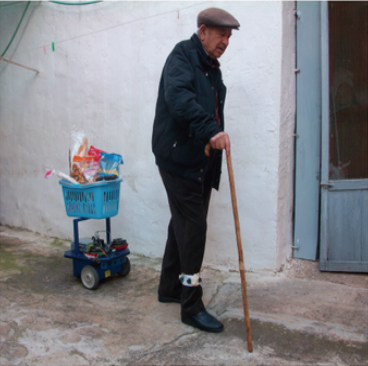
\includegraphics[width=0.4\textwidth]{figs/img/CompaRob}
   \caption{CompaRob Robot}
   \label{fig:CompaRob}
\end{figure}

In the current project, we are implementing XBee S2C RF radios, which are inexpensive and easily configurable, as a remote target device that is carried by the user. The robot will be able to track this remote instead of using line of sight methods~\cite{Miah2018-Intelligent}. In addition to the XBee S2C RF radios, we will equip the robot with a parabolic reflector, which improves radio reception at various distances and angles, \textit{i.e.,} angle of arrivals of RF signals from the remote, based on research done previously in this type of robot localization and mapping~\cite{Miah2018-Intelligent}~\cite{Li2013ANA}.


%----------------------------------------------------------------------
\section{Report Organization}
%----------------------------------------------------------------------
% \begin{itemize}
%     \item Chapter \ref{ch: intro} discusses the background and goals of the project and what other similar projects have accomplished.
%     \item Chapter \ref{ch: sysDesign} explains how the robotic cart system in this project is broken down fundamentally, the components used to build the robot, and the algorithms used to control the robot.
%     \item Chapter \ref{ch: implementation} discusses the implementation of all the parts onto the robot and the experimental results obtained when running the robot.
%     \item Chapter \ref{ch: conclusionAndFuture} concludes the project work and discusses future endeavors on this project.
%     \item Appendix \ref{ch: coppSimModeling} goes through the steps to model and simulate the Budget Bot chassis in CoppeliaSim
%     \item Appendix \ref{ch: assemblyInstructions} gives the step-by-step procedure for assembling the robot
% \end{itemize}

%%% Local Variables:
%%% mode: latex
%%% TeX-master: "../finalReport"
%%% End:

% %======================================================================
\chapter{System Design}
\label{ch: sysDesign}
%======================================================================

%----------------------------------------------------------------------
\section{System Block Diagram}
%----------------------------------------------------------------------
The overall system architecture of this project consists of two subsystems which
are the Mobile Cart and the Remote Target, which is held by the user or
customer, as shown in Fig. \ref{fig:sys_block_diag}. The proposed smart robotic
cart is a wheeled robot that sends and receives radio signals to follow the
remote target which acts as the beacon for the robotic cart system.

\vspace*{12pt}
\noindent
The high-level system block diagram of the proposed robotic cart (prototype) is shown in Fig. \ref{fig:sys_block_diag}. There are three inputs to the proposed cart system. The robotic cart is supplied with power through a battery that is mounted in the chassis of the robotic cart. There will be an on/off switch to allow the system to be powered down when not in use. This will save the battery from being drained by the XBees in the reflector array. The motion of the robotic cart is dependent on the motion of the remote.

\begin{figure}[H]
  \centering
  \includegraphics[width=\textwidth]{figs/systemBlockDiagram.pdf}
  \caption{System level block diagram detailing inputs and outputs to the
    robotic cart system.}
	\label{fig:sys_block_diag}
\end{figure}

\vspace*{12pt}
\noindent
The main output of the system is the position trajectory of the robotic cart in its environment. When the user moves with the remote target, the robotic cart is designed to follow the user.



%----------------------------------------------------------------------
\section{Subsystem Block Diagrams}
%----------------------------------------------------------------------
The Mobile Cart and the Remote Target subsystems are two separate operations
within the robotic cart system that run simultaneously. The two subsystems
communicate with one another by relaying radio messages between them. The first
block diagram is of the Remote Target subsystem shown in Fig.
\ref{fig:remote_block_diag}. Of the two subsystems the Remote Target is the
simplest since it only requires an XBee module attached to a 7.4V Li-Po battery
with a voltage regulation circuit since the XBee has a smaller input voltage of
3.3 volts. The two inputs for this system are the battery power and the incoming
RF messages which are passed through the RF transceiver Module and output the
outgoing RF messages.

\begin{figure}[H]
  \centering
  \includegraphics[width=\textwidth]{figs/remoteBlockDiagram.pdf}
  \caption{Remote Target block diagram}
  \label{fig:remote_block_diag}
\end{figure}

\vspace*{12pt}
\noindent
The Mobile Cart subsystem block diagram, shown in Fig.
\ref{fig:mobile_block_diag}, is the most complex of the two subsystems.The cart requires a power source, which will be a 7.4V, 8,000 mAh Li-Po battery since the
Li-Po works well with powering the embedded computer (BeagleBone Blue). The
power to the subsystem will be toggled by an on/off switch located on the
chassis of the robotic cart. The final input to the mobile cart subsystem is the
incoming RF signals. These incoming RF signals are passed to the direction
sensitive RF receivers which output the signals to the dual-direction
multiplexer. The dual-direction multiplexer then takes the four inputs from the
direction sensitive RF receivers and passes one output into the embedded
computer. Once the embedded computer gets these signals it can calculate the
localization and navigation algorithms and pass the information to the DC
motors.

\begin{figure}[H]
  \centering
  \includegraphics[width=\textwidth]{figs/mobileCartBlockDiagram.pdf}
  \caption{Block diagram showing the subsystem-level components of the proposed robotic cart.}
  \label{fig:mobile_block_diag}
\end{figure}

\vspace*{12pt}
\noindent
There are two outputs of the mobile cart subsystem. The first is the wheel velocities that move the cart and are passed from the DC motors. Lastly, the incoming RF signals are passed to our omnidirectional RF transceiver which outputs the outgoing RF signals.


%----------------------------------------------------------------------
\section{System Components}
\label{sec:System Components}
%----------------------------------------------------------------------

There are several components that are required for the mobile cart system.
Although some of these parts are available in the Bradley University laboratory,
other parts must be purchased. The parts that exist in the lab are listed in
\autoref{tab:Partslablist}. Also, \autoref{tab:Partslist} shows the list of
parts that were purchased. The parts compiled in the lists are the required
parts needed to build two smart robotic cart systems.

\begin{table}[H]
  \centering
  \caption{Parts Available in Laboratory}
  \begin{tabular}{c|c}
      \toprule
      \textbf{Quantity} & \textbf{Parts}\\
      \toprule
      2 & Budget Bot Chassis\\
      4 & 10 uF Ceramic Capacitor\\
      4 & LM1117 Regulator\\
      8 & 9V Batteries\\
      4 & Solderable PCB Boards\\
      3 & XBee USB Adapter\\
      \bottomrule
      %\multicolumn{2}{r|}{\textbf{Total}} & \$ 562.34\\
      %\bottomrule
  \end{tabular}
  %\caption{Parts Available in Laboratory}
  \label{tab:Partslablist}
\end{table}

\begin{table}[H]
  \centering
  \caption{Purchased parts for the Robotic Cart Project}
  \begin{tabular}{c|c|c}
    \toprule
    \textbf{Quantity} & \textbf{Parts} & \textbf{Price}\\
    \toprule
    4 & Pololu 37D Metal Gear motor 4751 & \$ 39.95\\
    12 & XBee S2C Module & \$ 23.10\\
    10 & XBee Adapter Board & \$ 4.99\\
    2 & Twotrees 4 Lead Nema 17 Stepper Motor & \$ 9.99\\
    1 & 4-Pin JST SH Connector - 20 Pack & \$ 7.99\\
    1 & 6-Pin JST SH Connector - 10 Pack & \$ 9.99\\
    1 & Aluminum Foil Tape - 2 in x 5 yd & \$ 6.05\\
    2 & Ovonic 7.4V 8000mAh LiPo Battery & \$ 40.99\\
    4 & Multiplexers & \$ 15.99\\
    \bottomrule
    \multicolumn{2}{r|}{\textbf{Total}} & \$ 562.34\\
    \bottomrule
  \end{tabular}
  %\caption{Purchased parts for the Robotic Cart Project}
  \label{tab:Partslist}
\end{table}

\vspace*{6pt}
\noindent
The main components for this project are the Budget Bot Chassis (Fig.
\ref{fig:budgetBotChassis}), the BeagleBone Blue embedded computer (Fig.
\ref{fig:beagleboneBlue}), and the XBee S2C Modules (Fig. \ref{fig:XBeeModule}).
Another major component is the reflector array that will be used to
directionally receive the RF signals from the remote target that is with the
user, which will be discussed in detail in the next section.

\begin{figure}[H]
  \centering
  \begin{subfigure}[t]{0.32\textwidth}
    \includegraphics[width=1\textwidth]{figs/img/budgetbot_chassis}
    \captionsetup{width=\textwidth}
    \caption{Budget Bot Chassis}
    \label{fig:budgetBotChassis}
  \end{subfigure}
  \begin{subfigure}[t]{0.32\textwidth}
    \includegraphics[width=1\textwidth]{figs/img/beaglebone_blue}
    \captionsetup{width=\textwidth}
    \caption{BeagleBone Blue}
    \label{fig:beagleboneBlue}
  \end{subfigure}
  \begin{subfigure}[t]{0.32\textwidth}
    \includegraphics[width=1\textwidth]{figs/img/Xbee-S2C-Module}
    \captionsetup{width=\textwidth}
    \caption{XBee S2C Module}
    \label{fig:XBeeModule}
  \end{subfigure}
  \caption{Main System Components}
\end{figure}

%----------------------------------------------------------------------
\section{Customized Reflector Array}\label{sec:customReflector}
%----------------------------------------------------------------------
The XBee RF modules that were used are omnidirectional. In this project, however, it is desired to have differences in the received signals based on the angle from which the signal is coming. Therefore, one of the major components of this project is the reflector array that enables the XBee modules to be direction sensitive. This section discusses the steps that were taken to construct such a reflector array.

\subsection{Reflector Design}
Two different models of reflector arrays were designed and constructed. The first design was a paraboloidal reflector with the focus on the antenna of the XBee module. The second design was a combination of a paraboloidal shape and a simpler parabolic shape. The motivation for each design will be discussed in sections \ref{subsec:paraboloidalReflector} and \ref{subsec:parabolicReflector}.

\subsubsection{Paraboloidal Reflector}\label{subsec:paraboloidalReflector}
The first design, shown in Fig. \ref{fig:paraboloidalReflector}, uses a reflector with a paraboloidal shape. This shape was selected since all signals entering the reflector parallel to the axis of the reflector will be focused at the focal point of the paraboloid. By mounting the XBee such that the center of the antenna coincides with the focal point of the paraboloid, the signal strength of the signals entering parallel to the axis will be maximized.
\begin{figure}
    \centering
    \includegraphics[width=3.5in]{figs/img/paraboloidalReflector.png}
    \caption{Purely Paraboloidal Reflector Array}
    \label{fig:paraboloidalReflector}
\end{figure}

\subsubsection{Combined Parabolic/Paraboloidal Reflector}\label{subsec:parabolicReflector}
The second design, shown in Fig. \ref{fig:parabolicReflector}, is the same on the lower half as the first design. However, the upper half is simply a surface where the horizontal cross-section is a parabola. The purpose for this design is similar to that of the first design, but the parabolic shape on the top will allow stronger detected signal strength of signals coming from above the reflector. Since the remote will be held by a person, it will generally be above the robot. The parabolic/paraboloidal reflector design is intended to allow better reception of signals from above.
\begin{figure}
    \centering
    \includegraphics[width=3.5in]{figs/img/parabolicReflector.png}
    \caption{Parabolic/Paraboloidal Reflector Array}
    \label{fig:parabolicReflector}
\end{figure}

\subsection{Reflector Construction}
With the recent advancements in 3D printing technology, it is not difficult to
create an object with a parabolic shape. In this project, the reflector dishes
were created using a 3D printer. The reflector array was designed to be modular,
where the dishes, top plate, and bottom frame were printed separately. After
printing, the dishes were lined with foil tape to provide the reflective surface
to focus the signals onto the antenna of the XBee. A layer of foil tape was also
placed on the top plate to provide a ground plane for the XBee. The parts were
then fastened together using M3 screws and nuts (Fig.
\ref{fig:reflectorConstruction}).
%
\begin{figure}[H]
    \centering
    \includegraphics[width=2.5in]{figs/img/reflectorConstruction.jpg}
    \caption{Reflector Construction}
    \label{fig:reflectorConstruction}
\end{figure}

%----------------------------------------------------------------------
\section{Localization and Navigation Algorithms}\label{sec:locAndNavAlgos}
%----------------------------------------------------------------------

This section illustrates the localization and navigation algorithms for the mobile cart to operate in an indoor/outdoor environment. The proposed robotic cart was modeled as a differential drive mobile robot (DDMR). The direction and distance of the remote relative to the cart are determined using a localization algorithm. This distance and angle are then passed to a navigation algorithm which calculates and applies the wheel speeds to move the robot toward the remote.

\subsection{Robot Model}\label{subsec:robotModel}
The robot used in this project was a differential drive mobile robot, which has
two drive wheels and a caster wheel for balance. The robot turns by applying
different speeds to the left and right wheels. As shown in Fig.
\ref{fig:robotGeometry}, the radius of the wheels is $R$, and the distance
between the wheels is $L$. The pose of the robot is given by the $x$-coordinate
($x$), the $y$-coordinate ($y$), and the orientation, ($\theta$), as shown in
Fig. \ref{fig:robotPose}. %
%
\begin{figure}[H]
    \centering
    \begin{subfigure}{0.3\textwidth}
        \centering
        \includegraphics[width=0.7\textwidth]{figs/robotGeometry.pdf}
        \caption{Robot Geometry}
        \label{fig:robotGeometry}
    \end{subfigure}%
    \begin{subfigure}{0.7\textwidth}
        \centering
        \includegraphics[width=0.7\textwidth]{figs/robotPose.pdf}
        \caption{Robot Pose}
        \label{fig:robotPose}
    \end{subfigure}
    \caption{Robot Model Parameters}
    \label{fig:robotModelParameters}
\end{figure}
%

\vspace*{12pt}
\noindent
Generally the robot is controlled by commanding a linear and angular speed ($v$ and $\omega$, respectively). These speeds must be converted into left and right wheel speeds. The following equations are used to calculate the angular left and right wheel speeds ($\omega_l$ and $\omega_r$, respectively):
$$\omega_l = \left(v - \omega\frac{L}{2}\right)\frac{1}{R}$$
$$\omega_r = \left(v + \omega\frac{L}{2}\right)\frac{1}{R}$$
To control DC motors in this way, the relationship between duty cycle and angular speed must be determined. Then the duty cycles to apply to the wheels can be calculated for the commanded $v$ and $\omega$.

\subsection{Localization Algorithm}
The localization algorithm is used to estimate the position of the remote with respect to the robot's local coordinate system. First the omnidirectional transceiver on top of the reflectors sends a signal strength request to the remote. The remote then replies with a message containing the strength of the signal it just received. This reply is detected by the receivers inside the reflectors as well as the omnidirectional transceiver. The strength detected by each of the directional receivers and the strength contained in the reply are then recorded. At this point, the entire reflector array is rotated 9\textdegree, and this process is repeated. The robot continues taking measurements in this way until the reflectors have been rotated one quarter turn. Since there are four reflectors at 90\textdegree to each other, a strength measurement has been recorded for every 9\textdegree increment around the robot. The angle of the remote is then estimated as the direction from which the strongest signal was received. The distance to the remote is calculated using the free-space path loss formula. The direction of reflector rotation is then reversed since the wires connecting the RF modules in the reflectors prevent the reflector from freely spinning. A flowchart of this algorithm is shown in Fig. \ref{fig:localizationAlgoFlowchart}.
\begin{figure}[H]
    \centering
    \includegraphics[width=3.5in]{figs/localizationAlgorithmFlowchart.pdf}
    \caption{Flowchart of Localization Algorithm}
    \label{fig:localizationAlgoFlowchart}
\end{figure}

\subsection{Navigation Algorithm}\label{subsec:navAlgo}
The navigation algorithm is used to drive the robot toward the remote. The inputs to the navigation algorithm are the angle to the remote ($\theta_r$) and the distance to the remote ($d_r$). A target point is then calculated as the point that is in the same direction as the remote, but closer to the robot by a fixed following distance ($d_{follow}$), as shown in Fig. \ref{fig:navAlgoDiagram}. The distance to the target point is calculated as $d_{tgt} = d_r - d_{follow}$, and the angle to the target point is $\theta_{tgt} = \theta_r$. The linear and angular speeds of the robot ($v$ and $\omega$, respectively) are then calculated using proportional control by the following equations:
$$v = K_vd_{tgt}$$
$$\omega = K_\omega\theta_{tgt}$$
The appropriate duty cycles are then calculated as specified in section \ref{subsec:robotModel} and applied to the wheel motors.
\begin{figure}[H]
    \centering
    \begin{subfigure}{0.45\textwidth}
        \centering
        \includegraphics[width=0.95\textwidth]{figs/navigationAlgorithmDiagram.pdf}
        \caption{Target Point Diagram}
        \label{fig:navAlgoDiagram}
    \end{subfigure}%
    \begin{subfigure}{0.55\textwidth}
        \centering
        \includegraphics[width=0.95\textwidth]{figs/navigationAlgorithmFlowchart.pdf}
        \caption{Flowchart}
        \label{fig:navAlgoFlowchart}
    \end{subfigure}
    \caption{Navigation Algorithm Details}
    \label{fig:navAlgoDetails}
\end{figure}

%%% Local Variables:
%%% mode: latex
%%% TeX-master: "../finalReport"
%%% End:

% %======================================================================
\chapter{Implementation}
\label{ch: implementation}
%======================================================================

Since this project was a new concept, the implementation had to start from scratch. Although there have been projects in the past that have used XBees to get signal strength, none of them used it in the same way as this project. For this project a mobile robot and a remote first had to be built to use for testing. Then a code base needed to be created to control the mobile robot according to the design algorithms.

%----------------------------------------------------------------------
\section{Robot Assembly}
\label{sec:Robot Assembly}
%----------------------------------------------------------------------

For this project, a Remote Target and Smart Robotic Cart were designed and implemented from off-the-shelf components.  As mentioned above in section \ref{sec:System Components}, some of the components were already available at Bradley University, and others had to be purchased specifically for this project. The parts are listed in \autoref{tab:Partslablist} and \autoref{tab:Partslist}.

\vspace*{12pt}
\noindent
Since the school already owned the Budget Bot chassis, it was a good choice for the base of the  Smart Robotic Cart. However, the Budget Bot chassis was modified slightly to work for this project. The main change was swapping out the motors that came with the Budget Bot for Pololu 27D Metal Gear motors since the original motors have a max speed of 212 RPM or 1.09m/s and the new motors have a max speed of 530 RPM or 2.72m/s when using the wheels with a diameter of 98mm. By switching out the motors enabled the robot to move faster to make it better able to achieve the goal of matching an average person's walking speed. The other modifications to the chassis were a hard power switch to directly cut off power to the XBee modules in the reflector and a power LED to indicate when this switch was on.

\vspace*{12pt}
\noindent
The next step was to attach the BeagleBone Blue microcomputer, XBee reflector array assembly, and breadboard to the top of the robot. A 2-cell LiPo battery was also installed inside the chassis of the mobile cart to provide power to the BeagleBone Blue directly and the breadboard through the switch. The power supplied to the breadboard is sent through a regulator circuit to drop it down from the 7.4V of the LiPo to 3.3V of the XBee. This circuit is also used on the remote which consists of a 7.4V LiPo battery and the XBee module with voltage regulator in between. This voltage regulator is built out of a LM117 regulator and a 10uF ceramic capacitor between the input and output pins of the regulator. The circuit diagrams for the robot and remote are shown in Figs. \ref{fig:robotCircuit} and \ref{fig:remoteCircuit}.
\begin{figure}[H]
    \centering
    \includegraphics[width=\textwidth]{figs/robotCircuit.pdf}
    \caption{Circuit Diagram for Robotic Cart}
    \label{fig:robotCircuit}
\end{figure}
\begin{figure}[H]
    \centering
    \includegraphics[width=0.7\textwidth]{figs/remoteCircuit.pdf}
    \caption{Circuit Diagram for Remote}
    \label{fig:remoteCircuit}
\end{figure}

\vspace*{12pt}
\noindent
The reflector array assembly from \autoref{sec:customReflector} was mounted on a stepper motor that was then attached to a 3D printed bracket. This bracket was then attached to the chassis using M3 screws. Another feature of this bracket is that it had a stop block built into the top  to allow the robot to automatically initialize the reflector array to the zero position when the robot starts up. This is accomplished by commanding a turn of 90\textdegree and allowing the reflectors to hit the stop block and be held there until this turn is complete.

\vspace*{12pt}
\noindent
The Xbee modules from the reflector array posed a bit of a problem when it came to connecting them to the BeagleBone Blue. The BeagleBone Blue has three standard UART ports and two others found in the USB and UART-GPS, which makes a total of five UARTs. Unfortunately not all five ports can be used to communicate with XBees since UART0 is used to provide communication with a computer through the console. Since port 0 is reserved for this function, the number of usable ports is only four, but the project requires communication with five XBees. The solution to this problem was to use two of the GPIO pins, two of the UART ports, and a dual 4-channel multiplexer. One of the UARTs can be directly connected to the top XBee, and the other UART can be routed through the multiplexer to the four side XBee modules. Then two UART ports are used to communicate with all five XBees.

\vspace*{12pt}
\noindent
Instructions for assembling the robot can be found in \autoref{ch: assemblyInstructions}. Therein, the sequence of steps is explained in detail with pictures to show the state of the robot. The finished prototype robot and remote are shown in Fig. \ref{fig:finishedPrototypes}.

\begin{figure}[H]
    \centering
    \begin{subfigure}[t]{0.5\textwidth}
        \centering
        \includegraphics[width=\textwidth]{figs/img/Finalized_robot.png}
        \captionsetup{width=\textwidth}
        \caption{Robotic Cart Prototype}
        \label{fig:overallPrototype}
    \end{subfigure}
    \begin{subfigure}[t]{0.35\textwidth}
        \centering
        \includegraphics[width=\textwidth]{figs/remote.pdf}
        \captionsetup{width=\textwidth}
        \caption{Remote Prototype}
        \label{fig:remotePrototype}
    \end{subfigure}
    \caption{Finished Prototypes}
    \label{fig:finishedPrototypes}
\end{figure}


%----------------------------------------------------------------------
\section{Code Base}
\label{sec:Code Base}
%----------------------------------------------------------------------

For the project some base functionality was needed to use with the main follower program so it could interact with the other components in the system. The BeagleBone Blue already has a set of ports on it that can be accessed and controlled using the Robot Control Library from Strawson Design ~\cite{Robot_Control_Library}.

\vspace*{12pt}
\noindent
Some custom libraries were built on top of the Robot Control Library to handle XBee Frames, AT Commands, and the stepper motor control. The XBee Frames library takes a given block of data containing the message and then packages it into a XBee Frame to send over UART to the XBee desired module. The XBee communications library also handles received messages from the XBee module and validates the received frame's integrity and extracts the message data from it. On top of the XBee communications library there is a library that generates AT Commands to package in the XBee Frames. The AT Command library also handles extracting response data from the AT Response Command structure and validates it.

\begin{figure}[H]
  \centering
  \includegraphics[width=\textwidth]{figs/img/Command Process Diagram.png}
  \caption{Process for XBee Communication over UART}
  \label{fig:CommandProcessDiagram}
\end{figure}

\vspace*{12pt}
\noindent
The final custom library is the stepper motor control library. This library had to be written since instead of using a dedicated stepper motor controller, two of the regular BBBlue DC motor control ports were used to power the stepper motor. The library handled translating how many steps to turn into the phase states to be sent to the DC motor ports that are connected to the stepper motor. The library also helped to keep track of basic information related to the stepper motor such as what its current angle should be.

%----------------------------------------------------------------------
\section{Experimental Results}
\label{sec:Experimental Results}
%----------------------------------------------------------------------

After the Robotic Cart, Remote Target, and code base were built, several different variants of the algorithms explained in \autoref{sec:locAndNavAlgos} were tested. There were two main types of variants tested. In one variant, the stepper motor is locked, preventing the reflector from rotating. In the other variant, the stepper motor is used to sweep through the angles.

\subsection{Rotating Reflector Tests}

The first type of test was where the robot would initialize the reflector array to the zero point with the stepper motor, then rotate in nine degree increments taking measurements as it went. A sweep ends when the motor has turned 81 degrees since at that point, with the four sides of the reflector, a full 360 degrees has been scanned.

\vspace*{12pt}
\noindent
This method offers a sufficiently dense set of data to base the angle predictions off of, but at the cost of having to wait until a entire sweep of the reflectors is completed for a single estimation of the remote location. The first attempt with this method was a simple test that would continuously sweep the reflectors and move the robot at the same time. Though this version did eventually make its way toward the remote, it had some errors in the robot's navigation trajectory. For example, the robot would correctly turn towards the remote, however, if it picked up a stronger signal from the XBee reverberations, it would drive off in a different direction. The robot would eventually find its way back into alignment and resume moving towards the remote.

\vspace*{12pt}
\noindent
The next version that used a rotating reflector, as well as the final version, works mostly the same as the first version, but with some improvements to the navigation. It was determined that the oscillations in the robot's trajectory in the first test were a result of turning the robot while also rotating the reflector. This adds additional rotation to the measurements in the global scope. Due to the design of the robot, the reflector array can only be rotated 90 degrees, but to properly fix this rotation issue the reflector array would need to be rotated more or less during a sweep to compensate for the robot's rotation. The solution was simply to alternate between sweeping the reflector and rotating the robot, all the while allowing the robot to always move forward. The rotation of the robot was limited to 15\textdegree before another measurement would be taken. In this version some additional windowed filters to average out the angle measurements were added, which did help to reduce the effects of random angles from noise in the system. Based on data collected in an anechoic chamber, offsetsfor each of the directional receivers were applied to try to convert the received signal strengths to use the same baseline. This offset was needed since each XBee would receive slightly different signal strengths when it was pointed directly at the remote.

\subsection{Locked Reflector Tests}

The locked reflector tests were run in between the first algorithm and the final algorithm which ultimately used a sweeping function to capture the XBee signals. The locked reflector algorithms were an attempt to reduce the time needed to get a set of measurements from the reflector by zeroing its rotation and then keeping it locked in the zero position. Since the data from this is relatively sparse, three different methods for estimating the angle of the remote were attempted. The first of these three methods was to try to select the direction that the signal was coming strongest from and then which of its two neighbor directions had the second strongest signal. With these two strengths the algorithm would then try to interpolate the angle based on the difference of the strengths between them. This method could possibly work, but due to the time constraints of the project, there was not enough time to implement and test this method.

\vspace*{12pt}
\noindent
The other two methods that were tried with the locked reflector were both different variants on machine learning algorithms. A small pool of data was collected both in an anechoic chamber and in a normal operating environment. The first algorithm attempted to use the K Nearest Neighbors algorithm to estimate the angle of the remote based on the relative signal strengths received by the directional XBees. The second algorithm used a neural network to predict the angle. Both of these algorithms failed to produce meaningful results, probably due to the fact that there was a very small pool of data to work with compared to the large amounts of data needed to perform machine learning algorithms. The noise in the signals proved too much for these algorithms to handle elegantly. If data were collected in many operating environments, machine learning techniques may be able to yield favorable results.

\subsection{System noise}

In both the fixed and sweeping experiments, an underlying issue was the amount of noise in the system. The first type of noise that occurs is noise from the multipath effect, where the signals bounce off obstacles in the environment, adding constructing and destructive interference randomly based on the robot's surroundings. The second source of noise was internal noise in the XBees, which was worse than what was expected. The XBee internal noise was isolated using an anechoic chamber where all the signals strengths did become stronger, but the base noise from the XBees persisted. The noise coming from the XBees tends to be about 2 to 6 dBm on average. The change from facing towards the remote then away from the remote is about 13 to 15 dBm. These ranges result in the occasional measurement that flip flops which reflector is actually facing the remote. The noise can be seen in the test measurements that were collected where 300 measurements were taken at several intervals around the robot as seen in Fig. \ref{fig:SensorDataGraphs}.

\begin{figure}[H]
    \centering
    \begin{subfigure}{0.50\textwidth}
        \centering
        \includegraphics[width=0.95\textwidth]{figs/img/Side1_Data.png}
        \label{fig:Side1Dat}
    \end{subfigure}%
    \begin{subfigure}{0.50\textwidth}
        \centering
        \includegraphics[width=0.95\textwidth]{figs/img/Side2_Data.png}
        \label{fig:Side2Dat}
    \end{subfigure}
        \begin{subfigure}{0.50\textwidth}
        \centering
        \includegraphics[width=0.95\textwidth]{figs/img/Side3_Data.png}
        \label{fig:Side3Dat}
    \end{subfigure}%
    \begin{subfigure}{0.50\textwidth}
        \centering
        \includegraphics[width=0.95\textwidth]{figs/img/Side4_Data.png}
        \label{fig:Side4Dat}
    \end{subfigure}
    \caption{Navigation Algorithm Details}
    \label{fig:SensorDataGraphs}
\end{figure}

\subsection{Distance}
This project initially planned to use the top XBee module's signal strength to determine the distance to the remote. In practice, however, it was determined to be nearly impossible with the current setup. The free-space path loss equation was used as a base equation to attempt to implement this feature in the project. One problem is that the free-space path loss formula is for use in free space, so it fails to yield the correct distance whenever any form of obstacle ends up in the line-of-sight path to the remote. The free-space path loss formula is also thrown off by any reflective surfaces around it due to the multipath effect. These issues could be potentially solved using a simultaneous localization and mapping algorithm such as EKF-SLAM.  Unfortunately, this approach would be very difficult since it relies on a known global reference point, but the robot in this project has no such global reference. It was decided that the distance measurement would be put on hold for future work on this project.

\section{Simulation using Robot Simulator}

Before constructing the physical robot prototype, a simulation was performed using a commercial robot simulator, CoppeliaSim. However, since RF signal behavior depends highly on the environment, the system could not be fully simulated. This section explains the steps taken to simulate the proposed robotic cart.

\vspace*{12pt}
\noindent
First, a model of the Budget Bot chassis was created in CoppeliaSim. The model is shown in Fig. \ref{fig:budgetBotModel}. The model was designed with the same dimensions as the physical chassis to accurately simulate the robot kinematics. Details on modeling a robot chassis in CoppeliaSim can be found in \autoref{ch: coppSimModeling}. Although \autoref{ch: coppSimModeling} explains the modeling of a robot chassis that is different than the Budget Bot chassis, the concepts are the same for modeling any robot chassis.
\begin{figure}[H]
    \centering
    \includegraphics[width=0.4\textwidth]{figs/img/budgetBotModel.png}
    \caption{Model of Budget Bot Chassis}
    \label{fig:budgetBotModel}
\end{figure}

\noindent
MATLAB code was written to control the simulation. The actual distance between the robot and the remote was measured, then random noise was added with a mean of 0 and a standard deviation of 0.07. This noisy measurement was then used in the navigation algorithm to determine how to drive the robot (see \autoref{subsec:navAlgo}). An image of the simulation is shown in Fig. \ref{fig:coppSimExample}, where the blue sphere represents the remote, and the green dot represents the target point.
\begin{figure}[H]
    \centering
    \includegraphics[width=0.5\textwidth]{figs/img/coppSimExample.png}
    \caption{CoppeliaSim Simulation}
    \label{fig:coppSimExample}
\end{figure}


%%% Local Variables:
%%% mode: latex
%%% TeX-master: "../finalReport"
%%% End:

% %======================================================================
\chapter{Conclusion and Future Work}
\label{ch: Chapter6}
\label{ch: conclusionAndFuture}
%======================================================================

%----------------------------------------------------------------------
\section{Conclusion}
%----------------------------------------------------------------------

This project shows that it is possible to use signal strength alone to make a mobile cart follow a remote target. A functional design for a mobile cart was developed and tested. In these tests, it was concluded that with the robot's current design, it would be extremely difficult to calculate an accurate distance to the remote from the signal strength alone. Therefore, the current design follows the target remote based on angle measurements alone. Due to the limitation of not having a usable distance value, the current implementation is unable to dynamically adjust its behavior based on proximity to the remote. One such planned parameter was the robot's velocity, which would have been reduced as the robot approached the remote target to prevent it from running into the user. Based on the literature review, it was determined that the Smart Robotic Cart design from this project is more cost-effective than most, if not all, of the existing solutions. It was shown that the robot could successfully track the remote target even when obstacles were obstructing the line-of-sight path between the robot and remote.

%----------------------------------------------------------------------
\section{Future Work}
%----------------------------------------------------------------------

Although the robotic cart prototype did successfully follow the remote based on signal strength alone, there is still much to be desired. The first item that would need to be addressed is a proper obstacle avoidance system. For the current robotic cart prototype, it was initially planned to have the robot avoid collision with the user by using the distance between the robot and remote, but this was dropped due to the inaccuracy of the distance measurement. This user avoidance could be incorporated into an obstacle detection and avoidance system in a future project, most likely using infrared or sonar sensors mounted on the robot. This is a necessary continuation of this project since, as it currently stands, it can detect and follow the remote through obstacles but will attempt to drive in a straight path towards the remote despite the obstacle between them.

\vspace*{12pt}
\noindent
The project also requires more overall tuning in any future work that is done on it. The two main places that need more tuning are the weights used to normalize the signal strengths out of the reflector array and the specs of the reflector array's design to optimize its performance. The values for normalizing the signal strengths coming out of the array currently are based on a relatively small and limited set of recorded data from the robot. For a future extension of this project, more measurements would be required to better determine the quality of the data coming out of each reflector. These values would most likely be obtained by taking many measurements in an anechoic chamber, which was also used for the current smaller set of sensor data. The data currently is only being used to calculate a base offset for each reflector's strength, though with enough data, it may be possible to use the top radio module's strength to adjust for overall degradation to the signal strength. The reflectors themselves also most likely need to be redesigned again. During testing, it was noted that the difference from facing the target to facing away from the target is only slightly greater than the average signal strength measurement noise.

\vspace*{12pt}
\noindent
Another problem that needs to be addressed in this project is determining a reasonably accurate distance measurement. The problem with distance stems from the fact that the locations remote and robot are relative to each other, so there is no global reference point that can be used to stabilize the measurements. The second problem is that the only way with the signal strength to get distance is to use a version of free-space path loss, which fails when the user stands between the remote and the robot. For this, two possible solutions were thought up after it was determined that signal strength alone would not work. These solutions were also determined to be outside the scope of what could be reasonably achieved within the allotted project time. The two possible solutions are to use signal strength with multi-frequency radio modules or to use the travel time of the message from the robot. The multi-frequency approach would still use signal strength but would potentially allow for a profile to be put together from the signal strength of each frequency to try and ignore the interference from objects. The other approach of using a message's travel time has been shown to work in such applications as GPS over large distances. This approach may work since the speed of the radio signal is generally less affected by objects in its path than signal strength is. The main challenge with this approach would be getting a sufficiently accurate time measurement for short distances. If either of these approaches to determining distance ended up working, then the algorithm could be more dynamic in its behavior and interpretation of the signal strengths.

%%% Local Variables:
%%% mode: latex
%%% TeX-master: "../finalReport"
%%% End:


% %----------------------------------------------------------------------
% % APPENDICES
% %---------------------------------------------------------------------- 
\appendix
% % Designate with \appendix declaration which just changes numbering style 
% % from here on
% % Add a title page before the appendices and a line in the Table of Contents
\addcontentsline{toc}{chapter}{APPENDICES} 
% %

% %======================================================================
\chapter{Modeling in CoppeliaSim}
\label{ch: coppSimModeling}
%======================================================================

%----------------------------------------------------------------------
\section{Problem Statement}
%----------------------------------------------------------------------
It is important to be able to simulate a robot's behavior before using the
actual robot to help find unexpected behaviors. CoppeliaSim is commercial robot
simulation software with the ability to simulate a robot that would operate in
exactly the way it would happen with a real robot. However, the robot of
interest is not currently included in CoppeliaSim's library that leads to
creating a model of the robot and simulating it before practical implementation.
The following sections explain how to model the Runt Rover robot in CoppeliaSim.

%----------------------------------------------------------------------
\section{Dimensions and 3D Modeling}
%----------------------------------------------------------------------
The Runt Rover robot is geometrically simple, with only a few dimensions being necessary to model the shape of the body and wheels. The dimensions used in this guide are shown in Fig. \ref{fig:runtRoverDims}

\begin{figure}
    \centering
    \includegraphics[width=3.5in]{figs/img/runtRoverDimensions}
    \caption{Dimensions of the Runt Rover Robot}
    \label{fig:runtRoverDims}
\end{figure}

The final 3D models are shown in Fig. \ref{fig:runtRoverModels}. An arrow was placed on the body to indicate orientation during simulation.

\begin{figure}
    \centering
    \begin{subfigure}[b]{0.6\textwidth}
        \centering
        \includegraphics[width=\textwidth]{figs/img/runtRoverChassis}
        \caption{Chassis}
        \label{fig:runtRoverChassis}
    \end{subfigure}
    \hfill
    \begin{subfigure}[b]{0.3\textwidth}
        \centering
        \includegraphics[width=\textwidth]{figs/img/runtRoverWheel}
        \caption{Wheel}
        \label{fig:runtRoverWheel}
    \end{subfigure}
    \caption{Modeled Parts}
    \label{fig:runtRoverModels}
\end{figure}

%----------------------------------------------------------------------
\section{Importing Models}
%----------------------------------------------------------------------
The next step is to import the 3D models into CoppeliaSim. This is accomplished using File \textgreater \ Import \textgreater \ Mesh. If the models were dimensioned in millimeters, the scale must be changed to 0.001 since CoppeliaSim uses meters. Since there are multiple colors in the models, there will be multiple shapes in CoppeliaSim. These can be grouped by dragging one shape onto another. Also, the shapes can be renamed. In modeling the Runt Rover, one chassis and four wheels are needed. The wheels must be placed in the correct locations on the axles.

%----------------------------------------------------------------------
\section{Adding Motors}
%----------------------------------------------------------------------
The robot can be given motors by means of revolute joints. These can be added using Add \textgreater \ Joint \textgreater \ Revolute. For the Runt Rover, one revolute joint was placed at each wheel. The joints should be named according to the wheel location since their names are used to interface the robot with Matlab. These joints are then made invisible by moving them to visibility layer 10. This is achieved in the Object Common Properties dialog box. The joints can be viewed by turning on visibility for layer 10 using the Layers dialog box. In the Object Properties dialog box, there is a button to open the Dynamic Properties dialog box. In this box, make sure the ``Motor enabled'' checkbox is enabled.

%----------------------------------------------------------------------
\section{Dynamic Shapes}
%----------------------------------------------------------------------
The 3D models do not have any dynamic properties within CoppeliaSim. It is recommended to use primitive shapes for the dynamic properties to reduce computation during simulation. For the Runt Rover, the wheels can be dynamically represented as cylinders, and the chassis can be dynamically represented as a cuboid. To add a primitive cylinder, use Add \textgreater \ Primitive Shape \textgreater \ Cylinder, and specify the size to be the same as a wheel. To add a cuboid, use Add \textgreater \ Primitive Shape \textgreater \ Cuboid, and specify the size to be the same as the chassis. These bodies must now be configured with the appropriate dynamic properties.

In the dynamic properties dialog box, make sure the ``Body is respondable'' checkbox is enabled, and enable the first four checkboxes and disable the last four checkboxes in the local respondable mask. Repeat this process on all of the dynamic shapes, alternating between selecting the first four and selecting the last four checkboxes in the local respondable mask. To give the robot mass and inertia, make sure the ``Body is dynamic'' checkbox is enabled, and click the ``Compute mass and inertia'' button. These dynamic shapes should be named according to the parts they represent (FrontLeftWheelDyn, for example). In the Object Common Properties dialog box, assign the dynamic shapes to visibility layer 9 to make them invisible.

%----------------------------------------------------------------------
\section{Linkage}
%----------------------------------------------------------------------
Now it is time to link everything together into one robot. First assign each graphical shape to its corresponding dynamic shape by dragging and dropping it onto the dynamic shape. Then assign the dynamic shapes for the wheels to the corresponding revolute joints in the same way. Finally, assign the revolute joints to the dynamic chassis. The name of the dynamic chassis is the name that will be used to interface with Matlab, so change it to ``RuntRover.'' Assign this shape to be the model base in the Object Common Properties dialog box. To make the bounding box the correct size, select the revolute joints and enable the ``Ignored by model bounding box'' and the ``Invisible during selection'' checkboxes in the Object Common Properties dialog box. Now enable the ``Select base of model instead'' checkbox for each of the visible objects. This allows us to select the entire robot by clicking on any part.

%----------------------------------------------------------------------
\section{Saving the Model}
%----------------------------------------------------------------------
To save this model, go to File \textgreater \ Save model as \textgreater \ CoppeliaSim model. The default location should be in the CoppeliaSim models directory. Create a new directory to contain your models and save the model within that directory. Your model will now be available in the CoppeliaSim library.


%%% Local Variables:
%%% mode: latex
%%% TeX-master: "../finalReport"
%%% End:

% %======================================================================
\chapter{Assembly Instructions}
\label{ch: assemblyInstructions}
%======================================================================

This appendix explains how to assemble the robot from the individual components. Some useful tools to have on hand during the assembly are a 2.5mm Allen key, a pair of needlenose pliers, a wire stripper, a scissors, and an exacto knife. Follow the steps below to assemble the robot.

\vspace*{18pt}
\noindent
\begin{Large}\textbf{Instructions}\end{Large}

\begin{enumerate}[label = \textbf{Step \arabic*.}]
    \item Get a Budget Bot Chassis (Fig. \ref{fig:assemblyBudgetBot}). For this project, a fuse, power switch, and power indicator LED were added to the Budget Bot Chassis. Install a 2-cell LiPo battery inside the Budget Bot. Route the balance plug and battery output cable up through the center hole on top of the Budget Bot.
    \begin{figure}[H]
        \centering
        \includegraphics[width=3.6in]{figs/img/assembly/01-BudgetBot.png}
        \caption{Modified Budget Bot Chassis}
        \label{fig:assemblyBudgetBot}
    \end{figure}

    \item Install a BeagleBone Blue and a solderless breadboard on the Budget Bot using 6mm M3 screws (Fig. \ref{fig:bbblueInstallation}, red circles). Connect the battery's balance plug to the terminal on the BBBlue, and the power output to the breadboard (Fig. \ref{fig:bbblueInstallation}, green circles). Finally, insert the motor cables into the breadboard (Fig. \ref{fig:bbblueInstallation}, blue circle).
    \begin{figure}[H]
        \centering
        \includegraphics[width=3.6in]{figs/img/assembly/02-bbblueInstallation.png}
        \caption{BBBlue and Breadboard Installation}
        \label{fig:bbblueInstallation}
    \end{figure}

    \item Connect the motor terminals to the motor output channels on the BBBlue (left: ch1, right: ch2) using two 2-pin JST-ZH connectors. Connect the motor encoders to the encoder channels on the BBBlue (left: ch1, right: ch2) using two 4-pin JST-SH connectors (Fig. \ref{fig:motorWiring}).
    \begin{figure}[H]
        \centering
        \includegraphics[width=3.6in]{figs/img/assembly/03-motorWiring.png}
        \caption{Motor Wiring}
        \label{fig:motorWiring}
    \end{figure}

    \item Prepare the stepper motor, the stepper motor bracket, four 6mm M3 screws, and four 8mm M3 screws (Fig. \ref{fig:stepperParts}).
    \begin{figure}[H]
        \centering
        \includegraphics[width=4in]{figs/img/assembly/04-stepperParts.jpg}
        \caption{Stepper Motor Parts}
        \label{fig:stepperParts}
    \end{figure}

    \item Insert four 6mm M3 screws through the holes on the top of the bracket and secure the stepper motor to the stepper motor bracket by threading the screws into the holes in the stepper motor (Fig. \ref{fig:stepperAssembly}). Make sure the motor connector comes out on the side of the bracket with the notch.
    \begin{figure}[H]
        \centering
        \includegraphics[width=4in]{figs/img/assembly/05-stepperAssembly.png}
        \caption{Mounting Stepper Motor onto Bracket}
        \label{fig:stepperAssembly}
    \end{figure}
    \pagebreak

    \item Insert four 8mm M3 screws through the holes in the feet of the bracket and secure the bracket to the Budget Bot (Fig. \ref{fig:stepperMounting}). Holes must be drilled in the Budget Bot Chassis to thread the screws into. Insert the stepper motor connector into the breadboard and tuck away the excess cable inside the Budget Bot.
    \begin{figure}[H]
        \centering
        \includegraphics[width=3.7in]{figs/img/assembly/06-stepperMounting.png}
        \caption{Mounting Stepper Motor onto Budget Bot}
        \label{fig:stepperMounting}
    \end{figure}

    \item Using two 2-pin JST-ZH connectors, connect motor output channels 3 and 4 to the stepper motor windings (Fig. \ref{fig:stepperWiring}).
    \begin{figure}[H]
        \centering
        \includegraphics[width=4in]{figs/img/assembly/07-stepperWiring.png}
        \caption{Stepper Motor Wiring}
        \label{fig:stepperWiring}
    \end{figure}
    \pagebreak

    \item Insert a DG409DJ+ multiplexer across the center of the breadboard (Fig. \ref{fig:multiplexer}). Make sure the divot is toward the end of the breadboard to prevent mistakes during the rest of the assembly.
    \begin{figure}[H]
        \centering
        \includegraphics[width=4.2in]{figs/img/assembly/08-multiplexer.png}
        \caption{Multiplexer Installation}
        \label{fig:multiplexer}
    \end{figure}

    \item Connect battery power to the multiplexer by connecting V+ to pin 14 and GND to pin 15 of the multiplexer (Fig. \ref{fig:multiplexerPower}).
    \begin{figure}[H]
        \centering
        \includegraphics[width=4.2in]{figs/img/assembly/09-multiplexerPower.png}
        \caption{Powering the Multiplexer}
        \label{fig:multiplexerPower}
    \end{figure}
    \pagebreak

    \item Insert an LM1117 3.3V regulator into the breadboard. Place a 10\textmu F capacitor between the output terminal and ground. Connect the ground terminal to the battery ground and the input power terminal to the battery V+ (Fig. \ref{fig:regulator})
    \begin{figure}[H]
        \centering
        \includegraphics[width=3.8in]{figs/img/assembly/10-regulatorWiring.png}
        \caption{Regulator Installation}
        \label{fig:regulator}
    \end{figure}

    \item Connect +3.3V from GPIO1 to pin 2 on the multiplexer (Fig. \ref{fig:multiplexerWiring}, red arrows). Connect GPIO1 pins 1 and 2 to multiplexer pins 1 and 16, respectively (Fig. \ref{fig:multiplexerWiring}, green and orange arrows). Connect UART1 TX and RX to multiplexer pins 8 and 9, respectively (Fig. \ref{fig:multiplexerWiring}, yellow and purple arrows). Finally, connect UART5 TX and RX into the breadboard (Fig. \ref{fig:multiplexerWiring}, blue arrows).
    \begin{figure}[H]
        \centering
        \includegraphics[width=4.8in]{figs/img/assembly/11-multiplexerBBBlueWiring.png}
        \caption{Connecting the Multiplexer to the BBBlue}
        \label{fig:multiplexerWiring}
    \end{figure}
    \pagebreak

    \item Prepare the reflector dishes, top plate, and bottom frame. Also prepare some 8mm and 10mm M3 screws and some M3 nuts (Fig. \ref{fig:reflectorParts}).
    \begin{figure}[H]
        \centering
        \includegraphics[width=4.4in]{figs/img/assembly/12-reflectorParts.jpg}
        \caption{Reflector Parts}
        \label{fig:reflectorParts}
    \end{figure}

    \item Insert an M3 nut into the slot at the top of one of the reflector dishes (Fig. \ref{fig:reflectorTopNut}).
    \begin{figure}[H]
        \centering
        \includegraphics[width=3.6in]{figs/img/assembly/13-reflectorTopNut.png}
        \caption{Top Reflector Nut}
        \label{fig:reflectorTopNut}
    \end{figure}
    \pagebreak

    \item Attach the top plate using an 8mm M3 screw (Fig. \ref{fig:reflectorTopPlate}).
    \begin{figure}[H]
        \centering
        \includegraphics[width=4.1in]{figs/img/assembly/14-reflectorTopPlate.jpg}
        \caption{Attaching Top Plate}
        \label{fig:reflectorTopPlate}
    \end{figure}

    \item Repeat steps 13 and 14 to attach all of the reflector dishes to the top plate (Fig. \ref{fig:finishedTopPlate}).
    \begin{figure}[H]
        \centering
        \includegraphics[width=4.1in]{figs/img/assembly/15-finishedReflectorTopPlate.jpg}
        \caption{Finished Top Plate}
        \label{fig:finishedTopPlate}
    \end{figure}
    \pagebreak

    \item Insert wires from the bottom of the reflectors up through the left slot (when viewed from above) and connect them to the VCC (red), DOUT (purple), DIN (yellow), and VSS (black) pins of an XBee adapter board (Fig. \ref{fig:topXBeeWiring}).
    \begin{figure}[H]
        \centering
        \includegraphics[width=4.2in]{figs/img/assembly/16-topXBeeWiring.jpg}
        \caption{Wiring for Top XBee}
        \label{fig:topXBeeWiring}
    \end{figure}

    \item Insert two M3 nuts into the slots on the underside of the top plate (Fig. \ref{fig:topXBeeNuts}).
    \begin{figure}[H]
        \centering
        \includegraphics[width=4.2in]{figs/img/assembly/17-topXBeeNuts.png}
        \caption{Nuts for top XBee}
        \label{fig:topXBeeNuts}
    \end{figure}
    \pagebreak

    \item Attach the XBee adapter board to the top plate using two 8mm M3 screws (Fig. \ref{fig:topXBeeMounting}).
    \begin{figure}[H]
        \centering
        \includegraphics[width=4.2in]{figs/img/assembly/18-topXBeeMounting.png}
        \caption{Mounting the Top XBee}
        \label{fig:topXBeeMounting}
    \end{figure}

    \item Insert wires through the back of a reflector dish and connect them to the VCC (red), DOUT (purple), DIN (yellow), and VSS (black) pins of an XBee adapter board (Fig. \ref{fig:sideXBeeWiring}). It is useful to number the purple and yellow wires at both ends with the reflector number. The reflectors should be numbered 1 through 4 going clockwise.
    \begin{figure}[H]
        \centering
        \includegraphics[width=4.2in]{figs/img/assembly/19-sideXBeeWiring.jpg}
        \caption{Wiring a Side XBee}
        \label{fig:sideXBeeWiring}
    \end{figure}
    \pagebreak

    \item Insert two M3 nuts into the underside of the support protruding from the reflector (Fig. \ref{fig:sideXBeeNuts})
    \begin{figure}[H]
        \centering
        \includegraphics[width=4.2in]{figs/img/assembly/20-sideXBeeNuts.png}
        \caption{Nuts for Side XBee}
        \label{fig:sideXBeeNuts}
    \end{figure}

    \item Mount the XBee adapter board using two 8mm M3 screws (Fig. \ref{fig:sideXBeeMounting}). Make sure the board is oriented such that the antenna of the XBee will be toward the reflective surface.
    \begin{figure}[H]
        \centering
        \includegraphics[width=4.2in]{figs/img/assembly/21-sideXBeeMounting.png}
        \caption{Mounting a Side XBee}
        \label{fig:sideXBeeMounting}
    \end{figure}
    \pagebreak

    \item Repeat steps 19 through 21 to mount XBee adapter boards into each of the four reflectors (Fig. \ref{fig:finishedSideXBees}).
    \begin{figure}[H]
        \centering
        \includegraphics[width=3.9in]{figs/img/assembly/22-finishedSideXBees.jpg}
        \caption{All Side XBees Mounted}
        \label{fig:finishedSideXBees}
    \end{figure}

    \item Wrap the wires coming from the reflector to keep them bundled into a single cable. Terminate the ends such that there is a 2-pin connector for +3.3V and GND (Fig. \ref{fig:reflectorWires}, red arrow), a 2-pin connector for the TX and RX to the top XBee (Fig. \ref{fig:reflectorWires}, blue arrow), a 4-pin connector for the TX pins of all four side XBees (Fig. \ref{fig:reflectorWires}, purple arrow), and a 4-pin connector for the RX pins of all four side XBees (Fig. \ref{fig:reflectorWires}, yellow arrow). Once again, it is useful to number both ends of the TX and RX wires to the side XBees.
    \begin{figure}[H]
        \centering
        \includegraphics[width=3.9in]{figs/img/assembly/23-reflectorWireEnds.png}
        \caption{Reflector Wire Ends}
        \label{fig:reflectorWires}
    \end{figure}
    \pagebreak

    \item Insert two M3 nuts into the slots at the bottom of a reflector (Fig. \ref{fig:bottomNuts}). The nuts should recess into a hexagonal slot that prevents them from rotating.
    \begin{figure}[H]
        \centering
        \includegraphics[width=3.6in]{figs/img/assembly/24-reflectorBottomNuts.png}
        \caption{Nuts for Bottom Frame}
        \label{fig:bottomNuts}
    \end{figure}

    \item Place the bottom frame onto the reflectors, with the stop plate pointed upward toward reflector 3. Route the wires through the hole between reflectors 1 and 2 (Fig. \ref{fig:reflectorWireRouting}).
    \begin{figure}[H]
        \centering
        \includegraphics[width=3.9in]{figs/img/assembly/25-reflectorWireRouting.png}
        \caption{Reflector Wire Routing}
        \label{fig:reflectorWireRouting}
    \end{figure}
    \pagebreak

    \item Attach the bottom plate to the reflectors using eight 10mm M3 screws (Fig. \ref{fig:bottomMounting}).
    \begin{figure}[H]
        \centering
        \includegraphics[width=3.6in]{figs/img/assembly/26-reflectorBottomMounting.png}
        \caption{Mounting the Bottom Frame}
        \label{fig:bottomMounting}
    \end{figure}

    \item Insert an XBee into each of the 5 XBee adapter boards (one on top and one in each reflector). Again, make sure that the XBees inside the reflectors are oriented with the antenna on the side toward the reflective surface (Fig. \ref{fig:XBeeInstallation}).
    \begin{figure}[H]
        \centering
        \includegraphics[width=3.6in]{figs/img/assembly/27-XBeeInstallation.jpg}
        \caption{XBee Installation}
        \label{fig:XBeeInstallation}
    \end{figure}
    \pagebreak

    \item Make sure the flat side of the stepper motor shaft is toward the back of the robot. Slide the reflector array onto this motor shaft, making sure the stop plate is pointed toward the back of the robot and is between the two stops on the stepper motor bracket (Fig. \ref{fig:reflectorMounting}).
    \begin{figure}[H]
        \centering
        \includegraphics[width=3.8in]{figs/img/assembly/28-reflectorMounting.png}
        \caption{Mounting the Reflectors on the Stepper Motor}
        \label{fig:reflectorMounting}
    \end{figure}

    \item Verify that the stop plate on the reflector array is between the stops on the stepper motor bracket (Fig. \ref{fig:installedReflector})
    \begin{figure}[H]
        \centering
        \includegraphics[width=3.8in]{figs/img/assembly/29-installedReflector.png}
        \caption{Reflector Stop Verification}
        \label{fig:installedReflector}
    \end{figure}
    \pagebreak

    \item Connect the reflector to the rest of the system by connecting the power cables to the output of the LM1117 regulator (Fig. \ref{fig:reflectorWiring}, red arrow), the top XBee TX and RX to the UART5 TX and RX (Fig. \ref{fig:reflectorWiring}, blue arrow), the side XBee TX wires to multiplexer pins 10 - 13 (Fig. \ref{fig:reflectorWiring}, purple arrow), and the side XBee RX wires to multiplexer pins 4 - 7 (Fig. \ref{fig:reflectorWiring}, yellow arrow). The side XBees should be connected to the multiplexer in order, with XBee 1 connecting to multiplexer pins 4 and 13.
    \begin{figure}[H]
        \centering
        \includegraphics[width=3.4in]{figs/img/assembly/30-reflectorWiring.png}
        \caption{Reflector Wiring}
        \label{fig:reflectorWiring}
    \end{figure}
\end{enumerate}

The robot assembly is complete! The fully assembled robot should look like the one shown in Fig. \ref{fig:assembledRobot}.
\begin{figure}[H]
    \centering
    \includegraphics[width=3.4in]{figs/img/assembly/31-assembledRobot.jpg}
    \caption{Assembled Robot}
    \label{fig:assembledRobot}
\end{figure}

%%% Local Variables:
%%% mode: latex
%%% TeX-master: "../finalReport"
%%% End:


% %----------------------------------------------------------------------
% % END MATERIAL
% %----------------------------------------------------------------------

% % B I B L I O G R A P H Y
% % -----------------------
% %
% % The following statement selects the style to use for references.  It controls the sort order of the entries in the bibliography and also the formatting for the in-text labels.
% \bibliographystyle{plain}
% % This specifies the location of the file containing the bibliographic information.  
% % It assumes you're using BibTeX (if not, why not?).
% \ifthenelse{\boolean{PrintVersion}}{
% \cleardoublepage % This is needed if the book class is used, to place the anchor in the correct page,
%                  % because the bibliography will start on its own page.
% }{
% \clearpage       % Use \clearpage instead if the document class uses the "oneside" argument
% }
% \phantomsection  % With hyperref package, enables hyperlinking from the table of contents to bibliography             
% % The following statement causes the title "References" to be used for the bibliography section:
% % \renewcommand*{\bibname}{References}
% Bibliography 
\renewcommand{\bibname}{Bibliography}

% Add the References to the Table of Contents
\addcontentsline{toc}{chapter}{\textbf{References}}

\bibliographystyle{IEEEtran}
\bibliography{bib/references.bib}
% Tip 5: You can create multiple .bib files to organize your references. 
% Just list them all in the \bibliogaphy command, separated by commas (no spaces).


%----------------------------------------------------------------------
\end{document}
%======================================================================



%%% Local Variables: 
%%% mode: latex
%%% TeX-master: t
%%% End: 
